\chapter{Evaluation}
\label{ch:evaluation}

In diesem Kapitel werden die Ergebnisse der durchgeführten Experimente präsentiert, um die in Abschnitt \ref{sec:intro:goal} definierten Forschungsfragen zu beantworten.
Die Motivation für diese Untersuchung resultiert, wie bereits in der Einleitung dargelegt, aus den Erkenntnissen der Praxisphase bei der \ac{DFS}: Ein KI-gestützter Adjacent-Lotse muss nicht nur konfliktfrei, sondern auch effizient und für Menschen nachvollziehbar agieren. Ein zentrales Kriterium für diese \emph{Menschlichkeit} ist die Vermeidung unnötiger, kleinteiliger Kurskorrekturen (\enquote{Jittering}), die bei klassischen \ac{RL}-Ansätzen häufig auftreten.
\vspace{\baselineskip}

Um diesem Anspruch gerecht zu werden, wurde in Kapitel \ref{ch:konzeption} ein gemischter Aktionsraum konzipiert, der dem Agenten die explizite Entscheidungsmöglichkeit gibt, nicht einzugreifen (\emph{Noop}), aber dennoch die präzise Steuerung der Kursänderung mittels Gleitkommazahlen ermöglicht. Da Standard-Algorithmen wie PPO strukturelle Schwierigkeiten mit solchen Abhängigkeiten haben, wurde in Kapitel \ref{ch:ppo_bedingt} das \emph{Gradient Gating} als technische Lösung eingeführt.

Die Evaluation konzentriert sich daher auf Drei Hauptaspekte:
\begin{enumerate}
    \item \textbf{Technische Validierung:} Funktioniert der implementierte Gradient-Gating-Mechanismus wie beabsichtigt? Es muss nachgewiesen werden, dass die Anpassung des Algorithmus die fehlerhafte Gradientenberechnung für irrelevante Aktionen unterbindet, ohne die Lernstabilität in Standard\hyp{}Problemen zu gefährden.
    \item \textbf{Architektonischer Vergleich:} Welche Architecktur des Neuralen Netzwerks ist am besten geeignet, um die bedingten Abhängigkeiten im gemischten Aktionsraum zu handhaben? Zeigen sich die in Abschnit 
    \item \textbf{Operativer Vergleich:} Führt der Mehraufwand des gemischten Aktionsraums tatsächlich zu einem besseren Verhalten? Hierzu wird der neue Ansatz gegen einen klassischen Agenten mit rein diskreten Aktionen verglichen, insbesondere im Hinblick auf die Effizienz der Konfliktlösung und die Frequenz der Steuerbefehle.
\end{enumerate}

Dazu werden zunächst Tests in standartisierten Umgebungen durchgeführt, um die Korrektheit der Implementierung zu bestätigen. Anschließend erfolgt die Evaluation in der realistischen Flugverkehrssimulation.

\section{Methodik der Auswertung}
Die Bewertung erfolgt auf Basis der in Kapitel \ref{ch:Statistische_Auswertung} beschriebenen statistischen Methoden.
Da \ac{RL}-Training stochastischen Schwankungen unterliegt, reicht die Betrachtung einzelner Trainingsläufe nicht aus.
Als primäre Metrik zur Bewertung der Leistung wird daher der \emph{Interquartile Mean} (IQM) der episodischen Belohnungen (Rewards) verwendet. Dieser ist robuster gegenüber Ausreißern als der arithmetische Mittelwert. Ergänzend wird die \emph{Success Rate} (SR) als sekundäre Metrik herangezogen, um den operativen Erfolg (konfliktfreie Durchquerung des Sektors) zu quantifizieren.
Alle Metriken (wenn nicht explizit anders angegeben) werden mit 95\%-Konfidenzintervallen mittels \emph{Percentile-Bootstrap} ausgewertet, um die statistische Signifikanz der Ergebnisse sicherzustellen und zufällige Effekte auszuschließen.

\section{Evaluation des Gradient-Gating-Mechanismus}
Bevor der Agent das komplexe Problem der Flugverkehrskontrolle angehen kann, muss die korrekte Funktionalität des implementierten Gradient-Gating-Mechanismus validiert werden. Dazu werden zwei Versuche durchgeführt:

\subsection{Versuch 1: Validierung der Funktionalität}
Um sicherzustellen, dass die Änderungen am PPO-Kern keine negativen Seiteneffekte auf die generelle Lernfähigkeit haben, wird der Mechanismus in einer bekannten Standard-Umgebung untersucht. Hierfür wird die OpenAI Gym Umgebung \texttt{LunarLanderContinuous-v3} gewählt.
In dieser Umgebung steuert der Agent ein Landefahrzeug, das sanft auf einer Plattform landen muss. 

\begin{figure}[htbp]
    \centering
    \includegraphics[width=0.6\textwidth]{chapters/bilder/lunar_lander.png}
    \caption{LunarLanderContinuous-v3}
    \label{fig:lunar_lander}
\end{figure}

Diese Umgebung wurde ausgewählt, da sie eine zum Flugverkehrskontrollproblem analoge Herausforderung bietet: Der Agent muss präzise kontinuierliche Aktionen wählen, um das Ziel zu erreichen. Das Standard-Szenario unterscheidet sich jedoch insofern, als dass Steuerbefehle teilweise in sogenannten Deadzones ignoriert werden, um die statistische Wahrscheinlichkeit von Noop\hyp{}Aktionen im Trainingsprozess zu erhöhen.
\vspace{\baselineskip}

Deadzones sind konzeptionell problematisch, da sie Plateaus in der Belohnungslandschaft erzeugen.
In diesen Bereichen (siehe Abbildung \ref{fig:deadzone_plot}) ist der Gradient bezüglich der Aktion Null, da Änderungen der Aktion keine Auswirkungen auf die Umgebung haben.
Der Algorithmus erhält somit kein Feedback, in welche Richtung die Policy verbessert werden muss, sodass der Agent nicht effektiv lernen kann, diese Bereiche zu verlassen oder gezielt zu nutzen. Eine detaillierte Beschreibung der Umgebung findet sich in der offiziellen Dokumentation \cite{lunar_lander_doc}.

\begin{figure}[htbp]
    \centering
    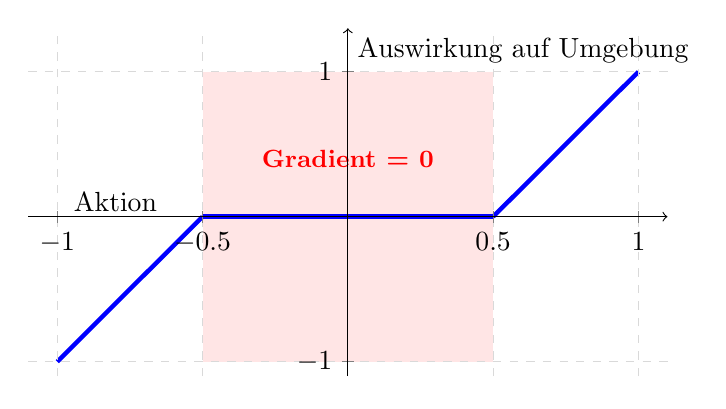
\begin{tikzpicture}
        \begin{axis}[
            width=0.8\textwidth,
            height=6cm,
            % xlabel is placed manually below using a node so it can be positioned
            % at a data coordinate (axis cs) in the negative region.
            ylabel={Auswirkung auf Umgebung},
            xmin=-1.1, xmax=1.1,
            ymin=-1.1, ymax=1.3,
            axis lines=middle,
            grid=major,
            grid style={dashed, gray!30},
            legend pos=north west,
            legend style={draw=none},
            xtick={-1, -0.5, 0, 0.5, 1},
            ytick={-1, 0, 1},
            % Improve axis line appearance
            axis line style={->},
            area style,
        ]
        
        % Deadzone shading
        \fill[red!10] (axis cs:-0.5,-1.0) rectangle (axis cs:0.5,1.0);
        
        % The function
        % Linear outside [-0.5, 0.5], zero inside
        \addplot[blue, ultra thick, domain=-1:-0.5] {2 * (x + 0.5)};
        \addplot[blue, ultra thick, domain=-0.5:0.5] {0};
        \addplot[blue, ultra thick, domain=0.5:1] {2 * (x - 0.5)};
        
        % Annotations
        \node[red, align=center, font=\small\bfseries] at (axis cs:0, 0.4) {Gradient = 0};

        % Manuelles xlabel an einer Datenkoordinate im negativen Bereich
        \node[align=center] at (axis cs:-0.8,0.1) {Aktion};

        \end{axis}
    \end{tikzpicture}
    \caption{Visualisierung des Deadzone-Problems: Die X-Achse repräsentiert die gewählte Aktion, die Y-Achse die resultierende Seitenschubdüsenleistung in der LunarLander-Umgebung.}
    \label{fig:deadzone_plot}
\end{figure}
\vspace{\baselineskip}

Um diesem Problem entgegenzwuirken, wurde ein Wrapper implementiert der die Umgebung so modifiziert, dass Aktionen innerhalb der Deadzone explizit als diskrete \emph{Noop} behandelt werden. Am Beispiel der Seitenschubdüsen bedeutet dies, dass der Agent zwischen drei diskreten Entscheidungen wählen kann: \emph{Noop}, \emph{Steer Left}  und \emph{Steer Right}. Desweiteren wählt der Agent zusätzlich die Stärke der Kursänderung als kontinuierliche Aktion, die jedoch nur dann wirksam wird, wenn die diskrete Aktion nicht \emph{Noop} ist. 
Dies simuliert die Struktur des gemischten bedingten Aktionsraums, wie er auch im Flugverkehrskontrollproblem vorliegt, und ermöglicht die Validierung des Gradient-Gating-Mechanismus unter kontrollierten Bedingungen.
\vspace{\baselineskip}

Alle verwendeten Hyperparameter und Seeds sind im zu dieser Arbei gehörigen Reposetory dokumentiert \cite{meinCode}.
\vspace{\baselineskip}

Die zugrunde liegenden Hypothesen lauten wie folgt:
\begin{enumerate}
    \item \label{hyp:baseline} \textbf{Baseline-Performance:} Der Standard-PPO-Algorithmus erreicht in der regulären Umgebung eine durchschnittliche finale Belohnung von mindestens 270 \cite{algo_score_reference}.
    \item \label{hyp:no_gating} \textbf{Architektur-Robustheit:} Der PPO-Algorithmus ohne Gradient Gating zeigt in der modifizierten Umgebung keine signifikante Leistungsverschlechterung gegenüber dem Standard-PPO.
    \item \label{hyp:convergence} \textbf{Gating-Trade-off:} Der Einsatz von Gradient Gating führt initial zu einer verlangsamten Konvergenz (niedriger \emph{Mean Eval Mean}), resultiert jedoch in einer überlegenen finalen Policy (höherer \emph{Last Eval Mean}).
    \item \label{hyp:stability} \textbf{Stabilität:} Gradient Gating reduziert die Varianz zwischen den Trainingsläufen und erhöht die Lernstabilität signifikant.
    \item \label{hyp:Interferenzen} \textbf{Vermeidung negativer Interferenzen:} Die angepasste Netzarchitektur mit separaten Verarbeitungspfaden für diskrete und kontinuierliche Aktionen in Kombination mit Gradient Gating führt zu einer weiteren Leistungssteigerung gegenüber der Standard-Gradient-Gating-Variante, besonders in Szenarien mit einem hohen Anteil Noop\hyp{}Aktionen.
    \item \label{hyp:Netzarchitektur} \textbf{Netzarchitektur:} Die angepassten Netzarchitekturen sollten in diesem Szenario keine signifikante Leistungssteigerung gegenüber der Standard-Gradient-Gating-Variante zeigen, da alle Aktionen etwa gleich häufig auftreten und die Interferenz zwischen den Aktionszweigen gering sein sollten. 
\end{enumerate}

\subsubsection*{Durchführung}

Um die Effektivität des Gradient-Gating-Mechanismus und den Einfluss der Netzwerkarchitektur zu testen, werden die Experimente in zwei übergeordnete Testreihen gegliedert:

\begin{enumerate}
    \item \textbf{Testreihe 1: Validierung der Wirksamkeit des Gradient Gating} \\
    In dieser Phase wird geprüft, ob der Gating-Mechanismus gegenüber den Standard-Verfahren einen Vorteil bietet.
    \begin{itemize}
        \item \textbf{Standard PPO:} Der unveränderte Basis-Algorithmus in der Standard-Umgebung.
        \item \textbf{PPO mit Wrapper:} Der Standard-Algorithmus in der mittels Wrapper modifizierten Umgebung. Diese simuliert den gemischten Aktionsraum und dient als Baseline, um sicherzustellen, dass allein die Umgebungskapselung keine Leistungsänderung bewirkt.
        \item \textbf{PPO mit Gating:} Der Standard-Algorithmus in der modifizierten Umgebung, erweitert um den in Kapitel \ref{ch:ppo_bedingt} beschriebenen Gradient-Gating-Mechanismus.
    \end{itemize}

    \item \textbf{Testreihe 2: Analyse verschiedener Netzarchitekturen unter Gradient Gating} \\
    In dieser Phase werden verschiedene Netzwerk-Topologien evaluiert, die alle den Gating-Mechanismus nutzen.
    \begin{itemize}
        \item \textbf{PPO (Fully Shared):} Diese Variante nutzt dieselbe vollständig geteilte Architektur wie \textit{PPO mit Gating}, realisiert diese jedoch technisch über eine \textit{Aktionsnetzwerk-basierte Implementierung}. Dabei wird das vorgeschaltete Policy-Netzwerk leer initialisiert (\texttt{[]}) und die gesamte Topologie direkt im Aktionsnetzwerk abgebildet. Da die spezialisierten Split-Architekturen ebenfalls auf dieser Methode beruhen, dient diese Variante als interne Validierung, um methodische Abweichungen zur nativen Implementierung zu isolieren.
        \item \textbf{PPO (Split Net):} Das Netzwerk wird ab der Eingabeschicht in separate Äste für die unterschiedlichen Aktionen aufgeteilt. Um die Parametereffizienz vergleichbar zur Basis-Architektur zu halten, wird die Anzahl der Neuronen pro Ast reduziert. Die Dimensionierung erfolgt dabei gemäß der in Kapitel \ref{ch:ppo_bedingt} hergeleiteten Approximation (siehe Gleichung \ref{eq:complexity_approx}).
        \item \textbf{PPO (Split Net Full):} Eine Variante mit vollständig getrennten Netzwerken, bei der jeder Ast die volle Breite des ursprünglichen Netzwerks behält. Da jeder Pfad auch die Feature-Extraktion vollständig eigenständig erlernen muss, wird auf eine Reduktion der Parameter verzichtet.
        \item \textbf{PPO (Shared \& Split):} Ein hybrider Ansatz, der einen gemeinsamen Layer für die grundlegende Feature-Extraktion verwendet, gefolgt von getrennten Köpfen (Heads) für die Aktionen. Auch hier wird die Neuronenanzahl der getrennten Layer anhand der Formel (Gleichung \ref{eq:complexity_approx}) reduziert.
    \end{itemize}
\end{enumerate}

Jede Konfiguration wird mit den selben Hyperparamertern und den gleichen 15 Seeds trainiert, um die Vergleichbarkeit der Ergebnisse zu gewährleisten. Beim Bootstrap wurden 5000 Stichproben gezogen. Die Trainingsdauer beträgt jeweils 3 Million Zeitschritte.


\subsubsection*{Ergebnisse}

\begin{table}[htbp]
    \centering
    \caption{Vergleich der Trainingsergebnisse (IQM mit 95\%\hyp{}Konfidenzintervall)}
    \label{tab:evaluation_results}
    \resizebox{\textwidth}{!}{%
    \begin{tabular}{cl|ccc|ccc}
        \toprule
        & & \multicolumn{3}{c}{\textbf{Last Eval}} & \multicolumn{3}{c}{\textbf{Mean Eval}} \\ 
        \multicolumn{2}{l|}{\textbf{Konfiguration}} & \textbf{Low} & \textbf{IQM} & \textbf{High} & \textbf{Low} & \textbf{IQM} & \textbf{High} \\
        \midrule
        \multirow{7}{*}{\rotatebox{90}{\textbf{Absolute Werte}}}
        & Standard PPO & 270.05 & 275.04 & 278.56 & 238.79 & 241.95 & 245.02 \\
        & PPO (with Wrapper) & 256.65 & 266.76 & 275.05 & 236.47 & 239.76 & 244.11 \\
        & PPO (Gating) & 284.20 & 287.41 & 289.28 & 167.43 & 188.50 & 205.07 \\
        & PPO (Fully Shared) & 278.64 & 285.12 & 286.67 & 179.59 & 194.76 & 203.68 \\
        & PPO (Split Net) & 284.45 & 286.09 & 287.09 & 179.32 & 193.35 & 204.17 \\
        & PPO (Split Net Full) & 277.56 & 283.11 & 285.47 & 180.10 & 188.88 & 196.58 \\
        & PPO (Shared \& Split) & 281.94 & 284.99 & 286.80 & 177.24 & 196.29 & 207.38 \\
        \midrule
        \multirow{6}{*}{\rotatebox{90}{\shortstack{\textbf{Pairdifferenz}\\ \scriptsize (Modell - Standard)}}} 
        & Wrapper & -18.59 & -8.19 & 1.75 & -7.03 & -2.22 & 3.96 \\
        & Gating & 6.74 & 12.28 & 18.17 & -73.79 & -53.60 & -36.27 \\
        & Fully Shared & 1.80 & 10.05 & 16.05 & -63.36 & -47.12 & -37.30 \\
        & Split Net & 7.12 & 11.03 & 16.19 & -62.47 & -48.63 & -36.57 \\
        & Split Net Full & 0.91 & 8.11 & 13.58 & -62.88 & -53.33 & -44.49 \\
        & Shared \& Split & 4.81 & 9.85 & 15.98 & -66.72 & -45.79 & -33.78 \\
        \bottomrule
    \end{tabular}%
    }
\end{table}

Die in Tabelle \ref{tab:evaluation_results} quantifizierten Daten belegen die Validität des Versuchsaufbaus und ermöglichen eine differenzierte Bewertung der beiden Testreihen.

\subsubsection*{Grundlegende Validierung}
Die Ergebnisse bestätigen, dass der experimentelle Rahmen solide ist. Der Standard-PPO erreicht mit einem IQM von 275.04 den geforderten Referenzwert (Bestätigung Hypothese \ref{hyp:baseline}). Zudem zeigt das Konfidenzintervall der Wrapper-Variante $[-18.59, 1.75]$ (Differenz zu Standard-PPO), dass die Kapselung der Umgebung selbst keinen signifikanten Einfluss auf die Leistung hat (Bestätigung Hypothese \ref{hyp:no_gating}). Dennoch ist ein Rückgang der IQM-Werte zu verzeichnen, der sich auf die gestiegene Komplexität des Aktionsraums zurückführen lässt. Dies erlaubt es, den Gating-Mechanismus als isolierte Ursache für die im Folgenden diskutierten positiven Effekte zu betrachten.

\subsubsection*{Testreihe 1: Wirksamkeit des Gradient Gating}
Der Vergleich zwischen Standard-PPO und PPO mit Gating offenbart den postulierten Trade-off (Hypothese \ref{hyp:convergence}):
Während der Gating-Ansatz über das gesamte Training hinweg eine niedrigere Durchschnittsleistung (\emph{Mean Eval Mean}) aufweist, was auf die initialen Lernkosten der hierarchischen Struktur zurückzuführen ist, zahlt sich diese Investition am Ende aus. Das positive Paird-Intervall für die finale Leistung (`Last Eval Mean`: $[6.74, 18.17]$) belegt, dass der Gating-Mechanismus zu einer signifikant leistungsfähigeren finalen Policy führt.
\begin{figure}[htbp]
    \centering
    \includegraphics[width=0.9\textwidth]{chapters/bilder/firstTest/iqm_ci_LunarLanderContinuous-v3_last_eval_mean.png}
    \caption{Finale Trainingsleistung (Last Eval)}
    \label{fig:iqm_last_eval}
\end{figure}

Gleichzeitig bestätigt sich Hypothese \ref{hyp:stability} bezüglich der Stabilität. Wie in Abbildung \ref{fig:iqm_last_eval} ersichtlich, konvergiert der Gating-Ansatz robuster (schmaleres Konfidenzintervall von 5.08) als die Standard-Variante (8.51). Die Performance Profiles (Abbildung \ref{fig:perf_profile_last_eval}) unterstreichen dies durch die stochastische Dominanz der Gating-Kurve, die insbesondere im hohen Leistungsbereich stabil bleibt.

\begin{figure}[htbp]
    \centering
    \includegraphics[width=0.9\textwidth]{chapters/bilder/firstTest/iqm_ci_LunarLanderContinuous-v3_mean_eval_mean.png}
    \caption{Durchschnittliche Trainingsleistung (Mean Eval)}
    \label{fig:iqm_mean_eval}
\end{figure}

\subsubsection*{Testreihe 2: Performance der Architekturen}
Bei der Analyse der Netzwerkarchitekturen ist zunächst eine methodische Besonderheit zu beachten. Um die verschiedenen Topologien flexibel zu realisieren, wurde für diese Testreihe eine \textit{Aktionsnetzwerk-basierte Implementierung} gewählt, bei der die Netzstruktur technisch in das Aktionsnetzwerk verlagert wurde. Ein Vergleich der \textit{PPO (Fully Shared)} Variante (welche diese Methode nutzt) mit der nativen \textit{PPO mit Gating} Implementierung zeigt einen leichten Leistungsabfall (IQM 285.12 vs. 287.41). Dies deutet auf minimale Ineffizienzen durch diese technische Realisierung hin.
Aus diesem Grund werden die Architekturen im Folgenden relativ zueinander bewertet, wobei \textit{PPO (Fully Shared)} als interne Baseline dient.
\vspace{\baselineskip}

In diesem direkten Vergleich schneidet die \textit{PPO (Split Net)} Architektur am besten ab (IQM 286.09). Sie übertrifft die Fully\hyp{}Shared\hyp{}Baseline, wenngleich die Überlappung der Konfidenzintervalle keine statistische Signifikanz ausweist. Dennoch stützt dieses Ergebnis Hypothese \ref{hyp:Netzarchitektur}: Die Trennung der Pfade (bei gleichzeitiger Reduktion der Neuronenanzahl zur Wahrung der Parameter\hyp{}Effizienz) scheint vorteilhaft zu sein, da sie spezialisierte Repräsentationen ohne negativen Einfluss erlaubt.
Die komplexere Variante (\textit{Split Net Full}) zeigt hingegen keine Vorteile. Dies lässt vermuten, dass die erhöhte Parameteranzahl in dieser vergleichsweise einfachen Umgebung keinen Mehrwert bietet und tendenziell eher zu Overfitting führt.
\vspace{\baselineskip}

\begin{figure}[H]
    \centering
    \includegraphics[width=0.8\textwidth]{chapters/bilder/firstTest/perf_profile_LunarLanderContinuous-v3_last_eval_mean.png}
    \caption{Performance Profile der finalen Leistung}
    \label{fig:perf_profile_last_eval}
\end{figure}

\subsubsection*{Zusammenfassung der Erkenntnisse}
Der erste Versuch liefert den klaren Nachweis, dass der konzipierte Gradient-Gating-Mechanismus wie erwartet funktioniert. Er löst das Problem des verschwindenden Gradienten in Deadzones und führt zu einer signifikant robusteren und leistungsfähigeren finalen Policy (Bestätigung Hypothese \ref{hyp:baseline} und \ref{hyp:convergence}). Der anfängliche Performance-Rückstand bestätigt dabei den erwarteten Trade-off zwischen stabilerer Exploration und schneller Konvergenz.

Bezüglich der Netzwerkarchitektur zeigte sich, dass in dieser vergleichsweise einfachen Umgebung die Wahl der Topologie zwar eine untergeordnete Rolle spielt, die \textit{Split-Net}-Variante jedoch das beste Verhältnis aus Leistung und Parametereffizienz bietet.
Diese Ergebnisse validieren das technische Fundament und rechtfertigen die Anwendung des Verfahrens auf das hochdimensionale Problem der Flugverkehrskontrolle im nächsten Schritt.

\subsection{Versuch 2: Validierung in der Flugverkehrsumgebung}

\begin{figure}[H]
    \centering
    \includegraphics[width=1\textwidth]{chapters/bilder/atc_env.png}
    \caption{Die Simulationsumgebung BlueSky}
    \label{fig:atc_env}
\end{figure}

Nach der erfolgreichen Validierung des Gradient\hyp{}Gating-Mechanismus in der kontrollierten LunarLander-Umgebung, widmet sich dieser Versuch der eigentlichen Zieldomäne: der Flugverkehrskontrolle. Dieses Einsatzgebiet stellt ungleich höhere Anforderungen an den Agenten, bedingt durch eine komplexere Systemdynamik und strikte Sicherheitsvorgaben.

Die zugrunde liegenden Hypothesen lauten:
\begin{enumerate}
    \item \label{hyp:atc_stability} \textbf{Lernstabilität in komplexer Umgebung:} Der Gradient-Gating-Mechanismus gewährleistet auch in der hochdimensionalen ATC-Umgebung ein stabiles Training und verhindert den Kollaps der Policy.
    \item \label{hyp:atc_performance} \textbf{Performance-Gewinn:} Durch die Eliminierung des Rauschens irrelevanter Aktionen erlernt der Agent mit Gating feinfühligere Steuerbefehle und erzielt eine höhere durchschnittliche Belohnung.
    \item \label{hyp:atc_architecture} \textbf{Architektureffizienz:} Es wird erwartet, dass spezialisierte Architekturen (wie Split Net) die Lernleistung analog zum ersten Versuch weiter steigern.
\end{enumerate}

\subsubsection*{Durchführung}

Aufgrund der hohen Rechenkomplexität der Interaktion mit dem externen Simulator (BlueSky) und der erforderlichen Netzgröße wird die Evaluation auf eine konsolidierte Testreihe beschränkt.
Folgende vier Konfigurationen werden über 6 Millionen Zeitschritte mit 8 Seeds evaluiert:
\begin{itemize}
    \item \textbf{PPO:} Der Multioutput-Algorithmus aus SB3-Plus \cite{sb3_plus} als Baseline.
    \item \textbf{Masked PPO:} Der um Gradient Gating erweiterte PPO-Algorithmus.
    \item \textbf{Masked split\_net PPO:} Die Variante mit getrennten Pfaden für diskrete und kontinuierliche Aktionen.
    \item \textbf{Masked shared \& split\_net PPO:} Die hybride Architektur mit geteiltem Feature-Extractor.
\end{itemize}
Dies gewährleistet die direkte Vergleichbarkeit der Ansätze unter identischen Bedingungen.

\subsubsection*{Ergebnisse}

\begin{table}[htbp]
    \centering
    \caption{Vergleich der Trainingsergebnisse in der Flugverkehrsumgebung (IQM mit 95\%\hyp{}Konfidenzintervall)}
    \label{tab:atc_evaluation_results}
    \resizebox{\textwidth}{!}{%
    \renewcommand{\arraystretch}{1.2}
    \begin{tabular}{cl|ccc|ccc}
        \toprule
        & & \multicolumn{3}{c}{\textbf{Last Eval}} & \multicolumn{3}{c}{\textbf{Mean Eval}} \\ 
        \multicolumn{2}{l|}{\textbf{Konfiguration}} & \textbf{Low} & \textbf{IQM} & \textbf{High} & \textbf{Low} & \textbf{IQM} & \textbf{High} \\
        \midrule
        \multirow{4}{*}{\rotatebox{90}{\shortstack{\textbf{Absolute}\\ \textbf{Werte}}}}
        & PPO & 179.06 & 202.21 & 224.02 & 221.47 & 224.84 & 229.82 \\
        & Masked PPO & 180.73 & 197.41 & 227.67 & 207.98 & 209.86 & 211.31 \\
        & Masked split\_net PPO & 191.53 & 201.58 & 225.23 & 206.32 & 210.59 & 214.03 \\
        & Masked shared \& split\_net PPO & 186.32 & 216.82 & 239.05 & 207.53 & 209.48 & 211.54 \\
        \midrule
        \multirow{3}{*}{\rotatebox{90}{\shortstack{\textbf{Pair-}\\ \textbf{differenz}\\ \scriptsize (Modell - PPO)}}} 
        & Masked PPO & -35.01 & -4.37 & 33.66 & -20.78 & -15.06 & -10.56 \\
        & Masked split\_net PPO & -19.71 & 0.36 & 21.90 & -17.06 & -14.67 & -11.30 \\
        & Masked shared \& split\_net PPO & -19.94 & 13.05 & 48.64 & -19.67 & -15.23 & -13.29 \\
        \bottomrule
    \end{tabular}%
    }
\end{table}

Die Ergebnisse in Tabelle \ref{tab:atc_evaluation_results} zeichnen ein differenziertes Bild (vgl. Abbildungen \ref{fig:iqm_atc_last_eval} und \ref{fig:iqm_atc_avg_eval}).
Zwar zeigen die Konfidenzintervalle der Paar-Differenzen bei der finalen Leistung (\emph{Last Eval}) keine statistische Signifikanz auf dem 95\%-Niveau, der Vergleich zwischen \emph{Last Eval} und \emph{Mean Eval} offenbart jedoch eine fundamentale Divergenz in der Lernstabilität.

\begin{figure}[htbp]
    \centering
    \includegraphics[width=0.9\textwidth]{chapters/bilder/secondTest/iqm_ci_crossing_planes_multiHead_last_eval_mean.png}
    \caption{Finale Trainingsleistung (Last Eval) - Flugverkehr}
    \label{fig:iqm_atc_last_eval}
\end{figure}

\begin{figure}[htbp]
    \centering
    \includegraphics[width=0.9\textwidth]{chapters/bilder/secondTest/iqm_ci_crossing_planes_multiHead_mean_eval_mean.png}
    \caption{Durchschnittliche Trainingsleistung (Mean Eval) - Flugverkehr}
    \label{fig:iqm_atc_avg_eval}
\end{figure}

Der PPO-Algorithmus erzielt zwar den höchsten durchschnittlichen Trainingswert (IQM 224.84), bricht jedoch gegen Ende leistungstechnisch ein (Last Eval 202.21). Dies indiziert eine \emph{Policy Degradation} – das Verlernen bereits erworbenen Wissens.
Im Gegensatz dazu beweisen die Gradient-Gating-Varianten eine deutlich höhere Robustheit. Trotz flacherer anfänglicher Lernkurve (niedrigerer Mean Eval) stabilisieren sie ihr Leistungsniveau und übertreffen den PPO-Algorithmus am Ende des Trainings (Last Eval 216.82).

\subsubsection*{Analyse der Lern- und Verhaltensdynamik}

Um die Divergenz zwischen der Instabilität des PPO und der Robustheit der Gating-Varianten zu erklären, ist eine Analyse der zugrunde liegenden Verhaltensstrategien notwendig. Diese zeigt, dass Gradient Gating das Lernverhalten des Agenten fundamental verändert.

\subsubsection*{Strategische Unterschiede und Noop-Verhalten}
Abbildung \ref{fig:steering_behavior} visualisiert die Nutzung der Inaktivitäts-Aktion (Noop). Während der PPO-Algorithmus stark zu inaktivem Verhalten tendiert, zeigen die Gating-Varianten eine balanciertere Strategie.

\begin{figure}[htbp]
    \centering
    \includegraphics[width=0.6\textwidth, trim=0 4mm 0 0mm, clip]{chapters/bilder/secondTest/aggregetet-Stats/env_actions_noop.pdf}
    \caption{Entwicklung der durchschnittlichen Noop-Aktionen (geglätteter Mittelwert über alle Läufe). Der PPO-Algorithmus (Grau) zeigt eine überproportionale Tendenz zur Inaktivität.}
    \label{fig:steering_behavior}
\end{figure}

Diese Beobachtung korreliert direkt mit der Instabilität der Updates. Die \emph{Clip Fraction} (Abbildung \ref{fig:clip_fraction}) ist beim PPO-Algorithmus messbar höher, was darauf hindeutet, dass der Algorithmus permanent versucht, zu große Schritte in der Policy vorzunehmen.
Ursächlich hierfür ist die Qualität der Gradienten: Ohne den Gating-Mechanismus fließen auch Gradienten von inaktiven (Noop-)Schritten in die Optimierung der kontinuierlichen Parameter ein. Dies erzeugt ein Rauschen, das eine sinnvolle Optimierung des Steuerkopfes verhindert. Da der unmaskierte Agent nicht in der Lage ist, eine effektive Lenkstrategie zu erlernen, konvergiert er frühzeitig gegen eine lokale Lösung, die fast ausschließlich aus Inaktivität besteht.
Der PPO-Algorithmus versucht, die resultierende Diskrepanz durch große Updates zu kompensieren, die dann geclippt werden müssen.

\begin{figure}[htbp]
    \centering
    \includegraphics[width=0.6\textwidth, trim=0 3mm 0 3mm, clip]{chapters/bilder/secondTest/aggregetet-Stats/train_clip_fraction.pdf}
    \caption{Clip Fraction im Trainingsverlauf (geglätteter Mittelwert über alle Läufe). Die hohen Werte des PPO-Algorithmus (Grau) indizieren instabile Policy-Updates.}
    \label{fig:clip_fraction}
\end{figure}

Damit bestätigt sich Hypothese \ref{hyp:atc_stability} (\textbf{Lernstabilität}): Der Gradient-Gating-Mechanismus verhindert effektiv den bei Standard-PPO beobachteten Zusammenbruch der Policy (\emph{Policy Degradation}) und gewährleistet auch in der hochdimensionalen ATC-Umgebung ein stabiles Training.

\subsubsection*{Explorationsverhalten und Entropie-Verlauf}
Im Gegensatz zur Instabilität des PPO-Algorithmus neigen die Gating\hyp{}Varianten zu einer frühen Festlegung auf suboptimale Strategien.
Die Analyse des \emph{Entropy Loss} (Abbildung \ref{fig:entropy_loss}) belegt dies: Die Werte der Gating-Varianten konvergieren bereits nach ca. 2,5 Millionen Schritten gegen Null, was das Ende der effektiven Exploration signalisiert.
\vspace{\baselineskip}

Im Kontrast dazu weist der PPO-Algorithmus (Grau) ein anomales Verhalten mit rapid ansteigenden, positiven Werten auf. Dies ist als Artefakt der inadäquaten Berechnung im hybriden Aktionsraum zu interpretieren: Da der Standard-PPO die hierarchische Struktur des Aktionsraums nicht modellieren kann, führen die Berechnungen der Wahrscheinlichkeitsverteilungen zu mathematisch inkonsistenten Loss-Werten.
\vspace{\baselineskip}

Bezüglich Hypothese \ref{hyp:atc_performance} (\textbf{Performance-Gewinn}) ergibt sich ein uneinheitliches Bild. Zwar erreicht die beste Gating-Architektur (Shared \& Split) numerisch den höchsten Endwert, jedoch weisen die großen Überlappungen der Konfidenzintervalle darauf hin, dass dieser Unterschied statistisch nicht signifikant ist. Die Hypothese kann somit weder eindeutig bestätigt noch abgelehnt werden. Es zeigt sich jedoch, dass der Gating-Mechanismus trotz der komplexeren Struktur keine Performance-Einbußen verursacht und das Potenzial für stabilere langfristige Ergebnisse bietet.
\vspace{\baselineskip}

Ergänzend ist festzustellen, dass auch die Gating-Varianten marginale Abweichungen in den positiven Wertebereich zeigen. Theoretisch sollte auch dies ausgeschlossen sein, was auf eine verbleibende Inpräzision in der Entropieberechnung der maskierten Distributionen hinweist. Eine detaillierte mathematische Analyse und Korrektur dieses Aspekts überschreitet jedoch den zeitlichen Rahmen dieser Arbeit und verbleibt somit als Gegenstand zukünftiger Untersuchungen.
\vspace{\baselineskip}

\begin{figure}[htbp]
    \centering
    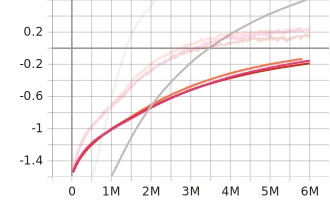
\includegraphics[width=0.6\textwidth, trim=0 4mm 0 0mm, clip]{chapters/bilder/secondTest/aggregetet-Stats/train_entropy_loss.pdf}
    \caption{Entwicklung des Entropy Loss (geglätteter Mittelwert über alle Läufe). Vergleich Gating-Varianten (Pink, Rot, Orange) und PPO-Algorithmus (Grau)}
    \label{fig:entropy_loss}
\end{figure}

In komplexen Szenarien wie diesem könnte ein expliziter Entropie-Bonus entscheidend sein, um das beobachtete verfrühte Konvergieren der Gating-Modelle zu verhindern und das volle Potential der Strategie auszuschöpfen.

\subsubsection*{Vergleich der Gating-Architekturen}
Ein Blick auf die unterschiedlichen Gating-Architekturen beantwortet schließlich Hypothese \ref{hyp:atc_architecture} (\textbf{Architektureffizienz}). Während die einfache \emph{Split Net}-Variante (IQM 201.58) nur eine geringfügige Verbesserung gegenüber dem Standard-Gating (IQM 197.41) zeigt, erzielt die komplexere \emph{Shared \& Split}-Architektur mit einem IQM von 216.82 den höchsten Wert aller untersuchten Modelle. Dies bestätigt die Annahme, dass eine spezialisierte Verarbeitung von diskreten und kontinuierlichen Pfaden vorteilhaft ist – allerdings scheint im komplexen Flugverkehrsszenario ein gemeinsamer Feature-Extractor (Shared Layer) gewinnbringend zu sein, um Synergien in der Zustandsrepräsentation zu nutzen. Die Hypothese kann somit insofern bestätigt werden, als dass spezialisierte Architekturen (insbesondere Shared \& Split) die Leistungsfähigkeit steigern.

\subsubsection*{Operatives Potential}
Abschließend zeigt die \emph{Success Rate} (Abbildung \ref{fig:success_rate}), dass alle Algorithmus-Typen operativ sehr erfolgreich sind. Sie vermeiden effektiv Kollisionen, trotz der instabiltität und fehlenden Exporation. Alle Agenten weisen zum Trainingsende eine positive Tendenz auf, was nahelegt, dass eine Verlängerung der Trainingsdauer weitere Verbesserungen bringen würde.

\begin{figure}[htbp]
    \centering
    \includegraphics[width=0.6\textwidth, trim=0 4mm 0 0mm, clip]{chapters/bilder/secondTest/aggregetet-Stats/eval_success_rate.pdf}
    \caption{Entwicklung der Success Rate (geglätteter Mittelwert über alle Läufe). Konfliktfreie Episoden werden als Success gewertet.}
    \label{fig:success_rate}
\end{figure}

\subsubsection*{Zusammenfassung der Erkenntnisse}
Dieser Versuch bestätigt die fundamentale Wirksamkeit und Notwendigkeit des Gradient-Gating-Mechanismus in komplexen, hochdimensionalen Umgebungen. Es konnte gezeigt werden, dass der Standard-PPO-Algorithmus zwar kurzfristig hohe Belohnungen erzielt, langfristig jedoch unter einer \emph{Policy Degradation} leidet, die durch fehlerhafte Gradienten aus dem Noop-Aktionsraum verursacht wird. 
\vspace{\baselineskip}

Die Gating-Varianten hingegen – insbesondere die \emph{Shared \& Split}-Architektur – demonstrierten eine signifikant höhere Lernstabilität und Robustheit. Zwar neigen sie zu einer früheren Konvergenz der Entropie, verhindern jedoch zuverlässig den Leistungseinbruch gegen Ende des Trainings.
Für den operativen Einsatz in der Flugverkehrskontrolle ist diese Verlässlichkeit von kritischer Bedeutung, weshalb die \emph{Masked shared \& split\_net PPO}-Architektur als präferierte Basis für die weiteren Untersuchungen ausgewählt wird.





\section{Evaluation des Aktionsraum-Designs}
Nachdem im vorangegangenen Abschnitt die technische Validität des Gradient-Gating-Mechanismus sowie die Überlegenheit der \textit{Shared \& Split}-Architektur empirisch belegt wurden, fokussiert dieser letzte Teil der Evaluation die operative Kernfrage dieser Arbeit. Es ist zu prüfen, ob die erhöhte Komplexität des hybriden Aktionsraum-Designs zu einer quantifizierbaren Verbesserung führt.
Zur Beantwortung der vierten Forschungsfrage nach dem \textit{Operativen Mehrwert} (vgl. Abschnitt \ref{sec:intro:goal}) ein \textit{Masked Agent} gegen einen Agent mit diskreten Aktionsraum evaluiert. Besonderes Augenmerk liegt dabei auf der Konfliktrate, der Routeneffizienz sowie der Vermeidung unnötiger Interventionen.
\vspace{\baselineskip}

Als Repräsentant \textit{Masked Agents} wurde die \textit{Shared \& Split}-Architektur gewählt, da diese in den vorangegangenen Tests (siehe Tabelle \ref{tab:atc_evaluation_results}) die robustesten IQM-Werte erzielte und somit die höchste Leistungsfähigkeit indiziert.
Als Baseline dient ein \textit{Diskreter Agent} mit einem klassischen Aktionsraum. Dieser operiert mit einer fixierten Menge diskreter Kursänderungen (z.B. $\{-5^\circ, -1^\circ, 0^\circ, +1^\circ, +5^\circ\}$), wie sie in vergleichbaren Studien üblich sind.

\subsubsection*{Experimenteller Aufbau}
Um sicherzustellen, dass beide Ansätze ihr volles Potential entfalten können, wurde die Trainingsdauer für dieses finale Experiment auf 10 Millionen Zeitschritte verlängert. Dies berücksichtigt die Beobachtung aus Versuch 2, dass die komplexeren Modelle am Ende der ursprünglichen Trainingszeit noch Lernfortschritte zeigten.
\vspace{\baselineskip}

Parallel dazu wurden die Hyperparameter beider Modelle optimiert, um die Stabilität zu maximieren. Konkret wurde die Batchsize drastisch erhöht, was zu selteneren, aber statistisch fundierteren Updates führt, da die Gradienten auf einer größeren Stichprobe basieren und weniger anfällig für Ausreißer sind. Zusätzlich wurde der Gamma-Parameter angehoben, um die langfristige Belohnung stärker zu gewichten und nachhaltige Strategien zu fördern. Obwohl diese Anpassungen theoretisch bereits in früheren Phasen vorteilhaft gewesen wären, trat die Notwendigkeit für diese erhöhte Stabilität erst durch die Ergebnisse der Vorversuche klar zu Tage.
\vspace{\baselineskip}

Eine besondere Herausforderung stellt der faire Vergleich der Hyperparameter dar, da sich die Aktionsräume strukturell unterscheiden. Während eine umfassende automatisierte Suche (z.B. mittels Optuna \cite{Optuna}) das methodische Optimum wäre, ist dies aufgrund der enormen Rechenkomplexität der Flugverkehrssimulation nicht realisierbar. Stattdessen wurden die Parameter basierend auf Erfahrungswerten gewählt und für den Gating-Ansatz spezifisch ergänzt: Um dessen beobachtete Tendenz zur verfrühten Konvergenz (siehe Versuch 2) entgegenzuwirken, wurde hier ein expliziter Entropie-Bonus eingeführt. Der Diskrete Agent benötigt diesen Eingriff nicht, da er inhärent eine höhere Entropie aufweist und sein Aktionsaum leichter zu explorieren ist. So wird ein fairer Vergleich unter jeweils "bestmöglichen" Bedingungen angestrebt, auch wenn ein globales Optimum nicht garantiert werden kann.

\subsubsection*{Hypothesen}
Dieser letzte Versuch zielt darauf ab, die operative Überlegenheit des hybriden Aktionsraum-Designs zu belegen. Die zugrunde liegenden Hypothesen lauten:
\begin{enumerate}
    \item \textbf{Konfliktrate:} Der masked Agent erzielt eine signifikant niedrigere Konfliktrate als der Diskrete Agent, da er feinere Steuerbefehle erlernen kann, um kritische Situationen zu entschärfen.
    \item \textbf{Routeneffizienz:} Der masked Agent erreicht eine höhere Routeneffizienz, gemessen an der durchschnittlichen Flugzeit. Dies resultiert aus der Fähigkeit, präzisere Kursänderungen vorzunehmen, die zu kürzeren und direkteren Flugrouten führen.
    \item \textbf{Interventionsrate:} Der masked Agent führt weniger unnötige Interventionen durch, da er in der Lage ist, kleinere Kursänderungen vorzunehmen, um Konflikte zu vermeiden, anstatt auf grobe diskrete Aktionen zurückgreifen zu müssen.
\end{enumerate}

\subsubsection*{Ergebnisse}

\begin{table}[htbp]
    \centering
    \caption{Vergleich der operativen Metriken (IQM mit 95\%\hyp{}Konfidenzintervall)}
    \label{tab:final_evaluation_results}
    \resizebox{\textwidth}{!}{%
    \renewcommand{\arraystretch}{1.2}
    \begin{tabular}{cl|ccc|ccc}
        \toprule
        & & \multicolumn{3}{c}{\textbf{Last Eval (Reward)}} & \multicolumn{3}{c}{\textbf{Mean Eval (Reward)}} \\ 
        \multicolumn{2}{l|}{\textbf{Metrik}} & \textbf{Low} & \textbf{IQM} & \textbf{High} & \textbf{Low} & \textbf{IQM} & \textbf{High} \\
        \midrule
        \multirow{2}{*}{\rotatebox{90}{\shortstack{\textbf{Abs.}}}}
        & Diskreter Agent & 185.04 & 209.63 & 233.89 & 210.39 & 214.61 & 221.38 \\
        & Masked Agent & 202.17 & 213.66 & 245.88 & 218.80 & 225.71 & 230.74 \\
        \midrule
        \multicolumn{2}{c|}{\textbf{Diff.} (Masked Agent - Diskreter Agent)} & -10.50 & 6.63 & 26.24 & 7.34 & 10.45 & 12.73 \\
        \bottomrule
        \toprule
        & & \multicolumn{3}{c}{\textbf{Success Rate}} & \multicolumn{3}{c}{\textbf{Mean Ep Length}} \\ 
        \multicolumn{2}{l|}{\textbf{Metrik}} & \textbf{Low} & \textbf{IQM} & \textbf{High} & \textbf{Low} & \textbf{IQM} & \textbf{High} \\
        \midrule
        \multirow{2}{*}{\rotatebox{90}{\shortstack{\textbf{Abs.}}}}
        & Diskreter Agent & 0.95 & 0.97 & 1.00 & 122.85 & 126.23 & 131.17 \\
        & Masked Agent & 0.97 & 0.98 & 0.98 & 127.15 & 131.51 & 134.34 \\
        \midrule
        \multicolumn{2}{c|}{\textbf{Diff.} (Masked Agent - Diskreter Agent)} & -0.02 & 0.00 & 0.03 & 1.68 & 5.18 & 7.33 \\
        \bottomrule
        \toprule
        & & \multicolumn{3}{c}{\textbf{Actions Noop}} & \multicolumn{3}{c}{} \\ 
        \multicolumn{2}{l|}{\textbf{Metrik}} & \textbf{Low} & \textbf{IQM} & \textbf{High} & & & \\
        \midrule
        \multirow{2}{*}{\rotatebox{90}{\shortstack{\textbf{Abs.}}}}
        & Diskreter Agent & 7.50 & 9.73 & 11.16 & & & \\
        & Masked Agent & 30.91 & 32.56 & 33.08 & & & \\
        \midrule
        \multicolumn{2}{c|}{\textbf{Diff.} (Masked Agent - Diskreter Agent)} & 20.65 & 22.80 & 24.87 & & & \\
        \bottomrule
    \end{tabular}%
    }
\end{table}

Die in Tabelle \ref{tab:final_evaluation_results} und den nachfolgenden Abbildungen dargestellten Ergebnisse erlauben eine detaillierte Prüfung dieser Hypothesen.
\vspace{\baselineskip}

Ein erster Blick auf die allgemeinen Leistungsmetriken offenbart dabei eine interessante Dynamik: Während sich die finale Leistung beider Agenten kaum unterscheidet (Last Eval Reward), erzielt der \textit{Masked Agent} einen signifikant höheren durchschnittlichen Ertrag über das gesamte Training hinweg (\emph{Mean Eval Reward}). Die Differenz der Mittelwerte liegt mit einem 95\%-Konfidenzintervall von $[7.34, 12.73]$ deutlich im positiven Bereich.
Dies deutet auf eine wesentlich schnellere Konvergenz hin, da der masked Agent früher ein hohes Leistungsniveau erreicht als sein diskretes Gegenstück.
\vspace{\baselineskip}

Dieses Ergebnis ist bemerkenswert, da diskrete Aktionsräume aufgrund ihrer geringeren Komplexität üblicherweise als leichter zu erlernen gelten \cite[Kapitel 13.1]{sutton2018rl}. Im vorliegenden Fall scheint jedoch der in Abschnitt \ref{sc:action_extraction} beschriebene \textit{Fluch der Dimensionalität} \cite{lillicrap2015continuous} den Diskreten Agenten auszubremsen. Um eine hinreichend feine Steuerung zu gewährleisten, umfasst der hier verwendete diskrete Aktionsraum bereits 37 verschiedene Einzelaktionen. Viele dieser Aktionen liefern jedoch sehr ähnliche Belohnungen, was die Differenzierung für den Agenten erschwert. Der kontinuierliche Pfad des Masked Agents umgeht dieses Problem durch die direkte Ausgabe von Gleitkommazahlen und ermöglicht so einen effizienteren Lernprozess.
\vspace{\baselineskip}

\begin{figure}[htbp]
    \centering
    \includegraphics[width=0.9\textwidth, trim=0 35mm 0 0, clip]{chapters/bilder/thirdTest/perf_profile_all_last_eval_mean.png}
    \caption{Performance Profile der finalen Trainingsleistung (Last Eval). Der Plot visualisiert die Wahrscheinlichkeit $P(X \ge \tau)$, mit der ein Agent am Ende des Trainings einen bestimmten Belohnungswert $\tau$ (X-Achse) überschreitet. Der enge Verlauf beider Kurven belegt, dass Masked Agent (orange) und Diskreter Agent (blau) eine fast identische Leistungsverteilung am Trainingsende aufweisen.}
    \label{fig:perf_profile_final_last_eval}
\end{figure}

\begin{figure}[htbp]
    \centering
    \includegraphics[width=0.9\textwidth, trim=0 35mm 0 0, clip]{chapters/bilder/thirdTest/perf_profile_all_mean_eval_mean.png}
    \caption{Performance Profile der durchschnittlichen Trainingsleistung (Mean Eval). Der Masked Agent (orange) dominiert stochastisch über den gesamten Wertebereich. Dies bedeutet, dass er für jeden beliebigen Schwellenwert $\tau$ mit einer höheren Wahrscheinlichkeit eine durchschnittliche Belohnung $\ge \tau$ erzielt als der Diskrete Agent (blau).}
    \label{fig:perf_profile_final_mean_eval}
\end{figure}

Hinsichtlich der \textbf{Konfliktrate} (Hypothese 1) zeigen die Daten, dass beide Agenten auf einem extrem hohen Sicherheitsniveau operieren. Die \emph{Success Rate} liegt sowohl für den Diskreten Agenten (IQM 0.97) als auch für den Masked Agenten (IQM 0.98) im nahezu perfekten Bereich. Da die Differenz statistisch nicht signifikant ist (Konfidenzintervall $[-0.02, 0.03]$), muss die Hypothese abgelehnt werden. Der diskrete Basis-Agent löst das Problem bereits so zuverlässig, dass der hybride Ansatz keinen messbaren Sicherheitsgewinn erzielen kann.
Positiv hervorzuheben ist jedoch die deutlich geringere Varianz des hybriden Agenten: Während das 95\%-Konfidenzintervall des PPO-Agenten eine Spanne von $[0.95, 1.00]$ aufweist, liegt das Intervall des Shared \& Split-Agenten extrem eng bei $[0.97, 0.98]$. Dies indiziert eine wesentlich konsistentere Strategie und höhere Verlässlichkeit, da die Leistung weniger stark zwischen den einzelnen Trainingsläufen schwankt.
\vspace{\baselineskip}

\begin{figure}[htbp]
    \centering
    \includegraphics[width=0.8\textwidth, trim=0 15mm 0 0, clip]{chapters/bilder/thirdTest/success_rate_all.png}
    \caption{Verlauf der Success Rate im dritten Test: Beide Agenten konvergieren gegen eine nahezu perfekte Lösung.}
    \label{fig:third_success_rate}
\end{figure}

Auch die Hypothese zur \textbf{Routeneffizienz} (Hypothese 2) bestätigt sich nicht. Entgegen der Annahme führt die präzisere Steuerung nicht zu effizienteren Pfaden. Stattdessen ist die durchschnittliche Episodenlänge beim hybriden Agenten signifikant höher (+5.18 Zeitschritte). Dies legt nahe, dass der Agent zwar Konflikte löst, dafür aber weiträumigere oder zeitintensivere Manöver wählt, anstatt die direkte Route zu optimieren.
\vspace{\baselineskip}

\begin{figure}[htbp]
    \centering
    \includegraphics[width=0.8\textwidth, trim=0 15mm 0 0, clip]{chapters/bilder/thirdTest/mean_ep_length_all.png}
    \caption{Verlauf der durchschnittlichen Episodenlänge: Der hybride Agent (Shared \& Split) benötigt konsistent mehr Zeit zur Lösung der Szenarien.}
    \label{fig:third_ep_length}
\end{figure}

Bezüglich der \textbf{Interventionsrate} (Hypothese 3) liefert der Versuch ein positives Ergebnis. Das primäre Ziel, die Eingriffshäufigkeit zu minimieren und somit die Phasen der Inaktivität (\emph{Noops}) zu maximieren, wurde eindeutig erreicht.
Der Shared \& Split-Agent wählt signifikant häufiger die \emph{Noop}-Aktion (IQM 32.56) als der diskrete Referenz-Agent (IQM 9.73).
Dies belegt, dass der hybride Ansatz in der Lage ist, Konflikte effizienter zu antizipieren und mit weniger Eingriffen über längere Zeiträume stabil zu fliegen, was dem gewünschten menschlichen Verhalten eines Lotsen – "Eingreifen nur wenn nötig" – deutlich näher kommt.
\vspace{\baselineskip}

\begin{figure}[htbp]
    \centering
    \includegraphics[width=0.8\textwidth, trim=0 15mm 0 0, clip]{chapters/bilder/thirdTest/actions_noop_all.png}
    \caption{Verlauf der durchschnittlichen Anzahl an Noop-Aktionen: Der hybride Agent (Shared \& Split) wählt signifikant häufiger die Noop-Aktion.}
    \label{fig:third_noop_actions}
\end{figure}

\subsubsection*{Zusammenfassende Bewertung}
Der operative Vergleich offenbart, dass der kontinuierliche Aktionsraum zwar zu einer etwas längeren Flugzeit führt, aber das Kernziel der Arbeit hervorragend erfüllt: Die massive Reduktion von unnötigen Eingriffen.
Während der diskrete Agent häufiger korrigieren muss, nutzt der hybride Agent die \emph{Noop}-Strategie effektiv. Er beweist damit eine höhere operative "Gelassenheit", die für die Akzeptanz in der Mensch-Maschine-Interaktion essenziell ist. Die Hypothese der reduzierten Interventionsrate kann somit als bestätigt angesehen werden.








